\setcounter{chapter}{1}

\chapter{Background}\label{cha:background}
This chapter reviews the background needed for our thesis. We explain all concepts, techniques, and tools that are used throughout this thesis. In Section \ref{sec:social-commitment-cha2}, the concept of social commitments as a means of communication between interacting agents is discussed. Section \ref{sec:knowledge-cha2} is devoted to briefly review reasoning about knowledge in MASs. In Section \ref{sec:system-models-cha2} some modeling formalisms including Interpreted Systems, we use in this thesis, are reviewed. Temporal logics for systems specification are also presented in this section. Section \ref{sec:Model-Checking-cha2}, describes the concept of model checking. Also, a review of some prominent existing model checkers is given in this section. Finally, we conclude this chapter in Section \ref{sec:summary-chap2}.


\section{Social Commitments} \label{sec:social-commitment-cha2}
The interoperability requirement in MASs has led to the introduction of various standardized agent communication languages (ACLs). The early proposals for defining the semantics of ACLs like KQML \cite{Finin1994} and FIPA ACL\footnote{See FIPA-ACL specifications (1997,1999,2001,2002), http://www.fipa.org/repository/aclspecs.php3} are developed using agent's mental states like beliefs, desires and intentions. These are now called mentalistic approaches because their focus are on the minds of the individuals participating in the interaction. A major weakness of these approaches is that they assume that \textit{agents can read each other minds} \cite{Singh1998}. Actually, in open environments where heterogeneous agents are made by different vendors and possibility using different technologies, it seems impossible to trust other agents completely or to make strong assumptions about their internal structure. This raises a serious verification problem for such approaches \cite{Singh2008,Wooldridge2009}. To overcome this drawback, some researchers took the initiative to think about other ways for defining ACLs  \cite{Singh1998}. As a result, social commitments have come to emergence. Social commitments are basically modeled as public information conveyed by an agent to another one. More specifically, a social commitment is an agreement between an agent, namely \emph{debtor}, to another agent, \emph{creditor}, in which the debtor engages towards the creditor to bring about a certain property \cite{Castelfranchi1995,Singh2005}.
%However, despite the fact that the term of \textit{social commitments} was constructed first by Castelfranchi in \cite{Castelfranchi1995}, the notion he introduced was not purely social because it is still analyzed in terms of the mental states of the partners.
In addition to being social, commitments are also public, and objective \cite{Colombetti2000}. These properties of social commitments help heterogeneous agents attribute the same meaning to the messages being exchanged so that the meaning is expressed using concepts that do not depend on an individual agent's internal structure. Importantly, a commitment between two agents is not just a static entity, but rather a dynamic one whose state changes over time as events occurs \cite{Akin2013,Torroni2009}. This dynamicity feature supports commitments' flexibility and can be captured through the manipulation of commitments via some operations such as \emph{creation}, \emph{fulfillment},
\emph{cancellation}, \emph{release}, \emph{assignment}, and
\emph{delegation} \cite{Singh1999}. In particular, a debtor may \emph{create} a commitment, thus activating it, or \emph{fulfill} a commitment, thus discharging it. However, for different reasons, a debtor might fail to fulfill its commitment; thus, it becomes violated. Given a commitment, its creditor can freely \emph{assign} it to another creditor, and its debtor may \emph{delegate} it to a another debtor. Furthermore, a debtor may \emph{cancel} a commitment; whereas, a creditor can \emph{release} the debtor from the commitment at any time.

%

%The notion of commitments as a foundation for understanding interactions among agents has been under development for about twenty years

Commitment-based approaches to ACLs have been around for about twenty years. Defining semantics of ACLs using the notion of social commitments has its roots back to the work of Singh \cite{Singh2000} in which he was the first to formalize a commitment-based ACL in temporal logic. Since then, social commitments have gained more and more popularity as a communication approach that makes no assumptions on the agents' internal states. To develop such approaches, various commitment logics that extend CTL (Computation Tree Logic), LTL (Lineal Temporal Logic), and CTL$^{*}$ (superset of CTL and LTL) have been introduced. Examples of efforts on this line can be found in
\cite{Bentahar2004,Giordano2007,Pham2007,Singh2000,Verdicchio2003}.
These logics have been successful in specification
and verification of systems from different areas such as
commitment-based protocols
\cite{Baldoni2010,El-Menshawy2010,Fornara2004b,Yolum2004},
modeling business processes \cite{Desai2009,Telang2009} and
agent-based web services \cite{Bentahar2008}.
However, the common limitation of theses proposals is that they neglect the uncertainty aspects of MASs and tend to assume typical behavior instead. In broad terms, uncertainty is a crucial aspect in MASs and has an impact not only on the behavior of the participating agents but also on the communication process that occur among these agents. %In Chapter \ref{cha:PCTLC}, we propose a new probabilistic logic whose primary purpose is to represent and reason about commitment-based agent communication in the presence of uncertainty.

In this thesis, we consider the notion of ``social commitments'' that is meant for communication. That is, the notion of commitments as a foundation for understanding interactions among agents. Therefore, we use communicative social commitments, also called illocutionary social commitments, as defined in \cite{Bentahar2012,El-Menshawy2013a}. Those commitments are formally denoted by $C_{i \to j} \varphi$, meaning that agent $i$, the debtor, commits to agent $j$, the creditor, to bring about $\varphi$, where $\varphi$ is the content of the commitment. Different notations with the same meaning can be found in \cite{Desai2009,Fornara2004a,Singh2000}.
This notion of ``social commitments'' should not be confused with some related notions such as ``Internal Commitments'', ``Norms'', and ``Obligations''. In traditional Artificial Intelligence (AI), a commitment was understood as the commitment of a single agent to some belief or to some course of action \cite{Levesque1990}. In this direction, ``internal commitment'' \cite{Castelfranchi1995,Singh2008} which refers to a commitment of an agent to itself has been widely used in the domain of AI. Norms, which are formal specifications of deontic statements that aim at regulating the interactions among agents, have also received a considerable attention in AI and MASs domains \cite{Balke2013,Singh2013,Testerink2013}. Obligations, on the other hand, have long been used as explicit mechanisms for influencing the behavior of interacting parties and providing some stability and reliability in their interactions \cite{Dignum2002}. Some researchers consider that commitments are somewhat like direct obligations \cite{Dignum1996,Singh2008}.

In contrast, the interesting feature that differentiates social commitments from the aforementioned notions is that a social commitment is directed from one party (the debtor) to another one (the creditor) which reflects the intuition that the debtor is committed to doing something for the creditor. These commitments are illocutionary in the sense that they are used as means of conveying information among interacting agents. Moreover, communicative commitments are equipped with a grounded semantics because the social accessibility relation has an intuitive and computational interpretation that makes its model checking possible.
%However, though Castelfranchi  tried to construct the notion of ``social commitment'', but it not purely social as it is yet analyzed in terms of the mental states of the partners \cite{Castelfranchi1995}. Another type of commitments introduced in AI before







\section{Reasoning about Knowledge} \label{sec:knowledge-cha2}

knowledge logics (also known as epistemic logics) are focused on reasoning about the knowledge that agents may have about themselves, the world, or other agents \cite{Fagin1995}. These logics have been shown to be a useful framework for the analysis of distributed algorithms and security protocols. Generally, an epistemic logic captures the essence of knowledge through modal operators. In this line, the contribution of Jaakko Hintikka in \cite{Hintikka1962} is recognized as the first attempt to investigate the logic of knowledge as a modal logic. Since then, researchers in AI and MASs have carried out numerous proposals to represent the evolution of knowledge \cite{Delgado2009,Fagin1995,Halpern2003,Huang2011,Lomuscio2007,Lomuscio2012,Meyer1995,Wan2013}. Formally, agent $i$ knows something is denoted by $K_i~\varphi$. From a verification perspective, model checking the logic of knowledge was first mooted by Halpern and Vardi \cite{Halpern1991}. Since that time theoretical aspects of model checking the logic of knowledge and its combinations with temporal logic have been studied. %Most existing solutions combine the logic of knowledge with LTL and/or CTL temporal logics.

In addition to reasoning about what one agent knows, it is often useful to be able to reason about the \textit{common knowledge}: the things that everyone knows, and that everyone knows that everyone knows, etc. Everyone knows can be defined as an abbreviation:

\noindent $E_G \varphi \equiv K_1 \varphi \wedge \dots K_n \varphi$, where $G$ is a group of agents, and $n$ is the number of agents in $G$.

\noindent The common knowledge operator $C_G$ is defined in terms of $E_G$ as follows:

\noindent $C_G \equiv E_G \varphi \wedge E_G^2 \varphi \wedge \dots \wedge E_G^k \wedge \dots $, where $E_G^k$ is read: ``everyone in $G$ knows $\varphi$ to degree k''.




\section{Modeling Techniques} \label{sec:system-models-cha2}
Transition Systems (TSs) are typically used as models to describe the behavior of systems \cite{Clarke1999}. They are the underlying models for all various non-real time models. TSs are modeled as directed graphs where nodes reflect the states, and edges represent the transitions. A state describes some information about the systems at a given moment of its behavior. Whereas, a transition describes how the systems can evolve from one state to another. A TS is a tuple $\mathbb{T} =(S, Act, \rightarrow, I, AP, \mathrm{L})$, where $S$ is a set of states, $Act$ is a set of actions, $\rightarrow\subseteq S\times Act \times S$ is the transition relation, $I\subseteq S$ is a set of initial states, $AP$ is a set of atomic propositions, and $\mathrm{L}: S \to 2^{AP}$ is a labeling function \cite{Baier2008}. %In Kripke structure \cite{Clarke1999}, $\mathrm{L}$ is introduced into TS to label states. However, in this section, we review some computational models that are used for modeling probabilistic systems.
In order to model random phenomena, transition systems are enriched with probabilities. This can be done in different ways. In the rest of this section, we review some probabilistic models that are used throughout our thesis.

\subsection{Interpreted Systems} \label{interpreted-systems-cha2}

The formalism of interpreted systems introduced by Fagin el al. \cite{Fagin1995} provides a useful framework to locally
model autonomous and heterogeneous agents who interoperate within
a global system via sending and receiving messages. This thesis builds on this formalism for various reasons:

\begin{itemize}
\item It is a suitable formalism for modelling agent-based systems as it provides a good level of abstraction that allows focusing more on modeling the key characteristics of the interacting agents along the evolution of their social commitments \cite{El-Menshawy2012}.
\item It has been successfully used to reason about various aspects of MASs such as time, knowledge, commitments, and correct behavior.
\item Interpreted systems are computationally grounded \cite{Wooldridge2000b}, meaning that the semantics of interpreted systems maps directly to the paths of the system, and vice-versa.
\item Interpreted systems can be easily extended. The original version introduced by Fagin et al. \cite{Fagin1995} has been extended in various ways as we will see below. This property of being readily extensible is important for us as we always need to extend it as required.
\end{itemize}

Suppose a set $\texttt{Agt}=\{1,\ldots,n\}$ of $n$
agents. At all times, each agent in the system is assumed to be in
some \textit{local} state, which intuitively records the complete
information that the agent can access at that time. Specifically,
each agent $i\in \texttt{Agt}$ is characterized by countable sets
$L_i$ and $Act_i$ of local states and actions respectively in
which the set $Act_i$ is mainly used to account for the temporal
evolution of the system. Also, local actions for each $i\in
\texttt{Agt}$ are performed in compliance with a local protocol
$\mathcal{P}_i: L_i\rightarrow 2^{Act_i}$, which assign a set
of enabled local actions to a local state. Intuitively, this set corresponds to the actions that are enabled in a given local state. Furthermore, the environment in which agents live may be modeled by means of a special agent $e$. Associated with $e$ are a set of local states
$L_e$, a set of actions $Act_e$, and a protocol $\mathcal{P}_e$. A
tuple $g = (l_1,\ldots, l_n,l_e) \in (L_1\times \ldots \times
L_n\times L_e)$ where $l_i\in L_i$ for each $i\in \texttt{Agt}$
and $l_e\in L_e$, is called a ``global state'' and represents the
instantaneous configuration of all agents in the system at a given
time (i.e., a snapshot of the global system at a specific time).

The local evolution function $\tau_i$ that determines the
transitions for an individual agent $i$ between its local states
is defined as follows:
%
\begin{equation}
\tau_i : L_i\times L_e\times Act_i \rightarrow L_i
\end{equation}
%
Similarly, the global evolution function of the system is defined as follows:
%
\begin{equation}
\tau : G\times ACT\rightarrow G
\end{equation}
%
where $ACT=Act_1 \times \ldots \times Act_n$ and each component
$a\in ACT$ is called a ``joint action'', which is a tuple of
actions (one for each agent), and $G = L_1\times \ldots\times
L_n\times L_e$ denotes a set of global states. The notation
$l_i(g)$ is used to represent the local state of agent $i$ in the
global state $g$. In addition, $I\in G$ is an initial global state
for the system. %For simplification, we remove the environment agent from the interpreted system formalism as done in \cite{Lomuscio2007}.

Bentahar et al. \cite{Bentahar2012} and El-Menshawy et al. \cite{El-Menshawy2013a} extended Fagin et al.'s formalism of interpreted systems with shared and unshared variables in order to account for communication that occurs during the execution of MASs and to provide an intuitive semantics for social commitments that are established through communication between interacting agents. They specifically associated with each agent $i\in \texttt{Agt}$ a countable set $Var_i$ of local
variables. Then, they used those variables to represent
communication channels through which messages are sent and
received. Technically, they denoted the value of a variable $x$ in
the set $Var_i$ at local state $l_i(g)$ by $l^{x}_i(g)$. Thus,
%
\begin{equation}
\textrm{if}~ l_i(g)=l_i(g'),~\textrm{then}~ l^{x}_i(g)
=l^{x}_i(g')~ \textrm{for~all}~ x \in Var_i
\end{equation}
%
The idea is that, for two agents $i$ and $j$ to communicate, they
should share a communication channel, which is represented by
shared variables between $i$ and $j$. In this perspective, a
communication channel between $i$ and $j$ does exist iff $Var_i
\cap Var_j \neq\emptyset$. For a variable $x \in Var_i \cap
Var_j$, $l^{x}_i(g)=l^{x}_j(g')$ means the values of $x$ in
$l_i(g)$ for agent $i$ and in $l_j(g')$ for agent $j$ are the same. This
intuitively represents the existence of a communication channel
between $i$ (in $g$) and $j$ (in $g'$) through which the variable
$x$ has been sent by one of the two agents to the other, and as a
consequence of this communication, $i$ and $j$ will have the same
value for this variable. The key point is that shared variables
are only used to motivate the existence of communication channels,
not the establishment of communication. Figure \ref{fig:social accessibility-cha2} depicts the idea of using shared and unshared variables for establishing communication channels between interacting agents.
The three conditions upon which a communication channel between $i$ and $j$ exists are listed below:

For each pair $(i,j) \in \texttt{Agt}^2$, $\sim_{i\rightarrow j} \subseteq S \times S$ is a social accessibility relation. $s \sim_{i\rightarrow j} s'$ is defined by the following conditions:
      %
  \begin{enumerate}
       \item $l_i(s)=l_i(s')$.
       \item $Var_i \cap Var_j \neq \emptyset$ such that $\forall x \in Var_i \cap Var_j$ we have $l^{x}_i(s)\!=\!l^{x}_j(s')$.
       \item $\forall y \in Var_j\!-\! Var_i$ we have $l^{y}_j(s)\!=\!l^{y}_j(s')$.
  \end{enumerate}

    %\begin{figure}[t]
    \begin{figure}[!ht]
                \begin{center}
                \includegraphics[width=12cm, %height=7cm]{chap2/img/social-accessibility-cha2.eps}
                height=7cm]{chap2/img/social-accessibility1.eps}
                \end{center}
                \caption{Social accessibility relations as defined in \cite{Bentahar2012,El-Menshawy2013a}}
                \label{fig:social accessibility-cha2}
    \end{figure}

Recently, Al-Saqqar et al. \cite{Al-Saqqar2014a} have modified the definition of social accessibility relations given in \cite{Bentahar2012,El-Menshawy2013a} in such a way that the new definition does no longer depend on the unshared variables but rather depends merely on the shared variables between the interacting agents as shown in Figure \ref{fig:modified social accessibility-cha2}. The new condition upon which a communication channel is established is stated below:

 $ s \approx_{i \rightarrow j} s' $ iff $ Var_i \cap Var_j \neq \emptyset $ such that $ \forall x \in Var_i \cap Var_j $ we have $ l_i^x(s) =
l_i^x(s') = l_j^x(s')$, where $\approx_{i\rightarrow j} \subseteq S \times S$ is the new social accessibility relation \cite{Al-Saqqar2014a}.

%\begin{figure}[t]
    \begin{figure}[!ht]
                \begin{center}
                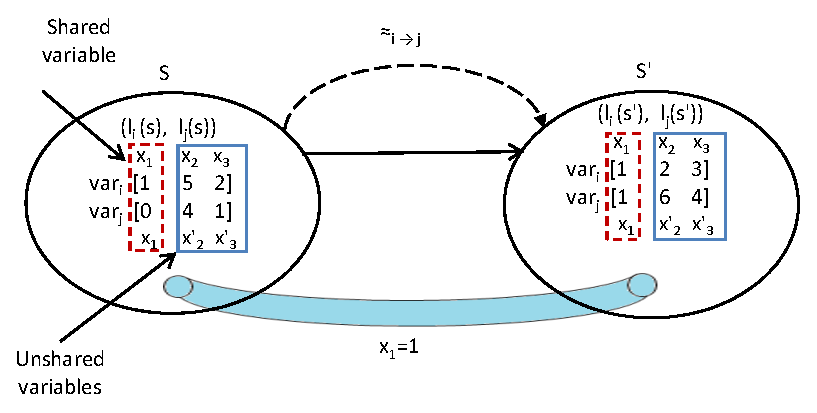
\includegraphics[width=12cm, height=7cm]{chap2/img/social-accessibility2.eps}
                \end{center}
                \caption{The modified version of social accessibility relations as in \cite{Al-Saqqar2014a}}
                \label{fig:modified social accessibility-cha2}
    \end{figure}


The original version of interpreted systems formalism was also extended by Halpern et al. \cite{Halpern2003} and further by Wan et al. \cite{Wan2013} to model the stochastic behavior of MASs. Accordingly, the local evolution function is defined as follows:
%
\begin{equation}
\tau_i: L_i \times Act_i \times L_i \rightarrow[0,1]
\end{equation}
%
such that for all $l_i \in L_i$, we have $\sum_{l'_i\in L_i}
\tau_i(l_i,a^{l_i\rightarrow l'_i},l_i')=1$ wherein
$a^{l_i\rightarrow l'_i}$ is the local action labeling a
transition between local states $l_i$ and $l'_i$ of agent $i$.


Moreover, the global evolution function is defined as follows:
%
\begin{equation}
\tau: G \times ACT \times G \rightarrow[0,1]
\end{equation}
%
%This function satisfies Markovian properties in the sense that
The sum of the probabilities over all possible transitions from a given state $g$ must be $1$: for all $g \in G$, $\sum_{\substack{g'\in G}}
\tau(g,a^{g\rightarrow g'},g')=1$ where $a^{g\rightarrow g'}$ is
the action labeling the transition between the two global states
$g$ and $g'$ of the system.

Such a modified version of the interpreted systems formalism is
called \textit{probabilistic interpreted systems}
\cite{Halpern2003}. In the formalism of probabilistic interpreted
systems, the transition probability matrix can be computed by
\cite{Wan2013}:

\begin{equation}\label{global-evo-fun}
\tau(g,a^{g\rightarrow g'},g')= {\prod_{\substack{i \in
\texttt{Agt}}} \tau_i(l_i(g), a^{l_i(g) \rightarrow
l_i(g')},l_i(g'))}
\end{equation}




\subsection{Discrete Time Markov Chains (DTMCs)} \label{sec:DTMC-cha2}

DTMCs are commonly used as models for probabilistic systems. A DTMC is a transition system that defines the probability of moving from one state to another.
\begin{definition}[DTMC]\label{def:DTMC}
Given a set of atomic propositions $AP$, a DTMC can be defined as a 4-tuple
$\mathbf{D}$ = $(S,\overline{s},\mathbf{P},L)$ where:

\begin{itemize}
  \item  $S$ is a nonempty and finite set of states;
  \item  $\overline{s}$ is the initial state;
  \item  $\mathbf{P} :  S\times S\rightarrow[0,1]$ is the transition
  probability matrix, such that for every state $s\in{S}$, we have
  $ \sum_{s' \in{S}} \mathbf{P}(s,s' )=1$;
  \item  $L : S\rightarrow 2^{AP}$  is a labelling function which assigns to each state $s \in S$ the set $L(s)$ of atomic propositions that are valid in the state.
\end{itemize}
\end{definition}


DTMCs are stochastic models of systems that change their states at discrete-times $(n=0,1,2,\dots)$ and have the following property: if the system enters state $s$ at time $n$, it stays there for exactly one unit of time and then jumps to state $s'$ at time $n+1$ with probability $\mathbf{P}(s, s')$, regardless of its history up to and including time $n-1$ \cite{Kulkarni1995}. The definition shows that states are labelled with atomic propositions which indicate the status of the system (e. g., waiting, sending). The system can change its states according to a probability distribution given by the transition probability matrix $\mathbf{P}$. Each element $\mathbf{P} (s,s')$ of the transition probability matrix gives the probability of making a transition from state $s$ to state $s'$. A transition from state $s$ to $s'$ can only take place if $\mathbf{P}(s, s') > 0$. However, if $\mathbf{P}(s, s') = 0$, no such transition is possible. Again, the probabilities from a given state must sum up to 1, i.e. $\sum_{s' \in{S}} \mathbf{P}(s,s' )=1$.


\subsection{Markov Decision Processes (MDPs)} \label{sec:MDP-cha2}
MDPs can be seen as transition systems in which in any state a nondeterministic choice between probability distributions exists.

\begin{definition}[MDP]\label{def:MDP}

Given a set of atomic propositions $AP$, an MDP model $\mathbf{M}$ can be defined as a 5-tuple, $\mathbf{M}$ = $(\mathbb{S}, AC, \textsf{P}_t ,I_i, L)$, where:

\begin{itemize}

  \item  $\mathbb{S}$ is a nonempty and finite set of states.

  \item  $\textsf{P}_t:  \mathbb{S}\times AC\times \mathbb{S}\rightarrow[0,1]$ is the transition probability function, such that for every state $s\in{\mathbb{S}}$ and action $\theta \in AC$, we have $\sum_{s' \in{\mathbb{S}}} \textsf{P}_t(s,\theta ,s') \in \{0,1\}$.

  \item  $AC $ is a set of actions. At state $s \in \mathbb{S}$, the action $\theta$ is enabled iff $\sum_{s' \in{\mathbb{S}}} \textsf{P}_t(s,\theta ,s')=1$.

  \item  $I_i$ is an initial state.

  \item  $L : \mathbb{S}\rightarrow 2^{AP}$  is a state labeling function.
\end{itemize}
\end{definition}

MDPs possess the Markov property, which requires that any information necessary to predict the effects of all events is captured in the state. In other words, the effects of an event in a state depend only on that state and not on the prior history. However, the major difference between MDPs and DTMCs is the choice of actions. While a DTMC describes the state transitions of a stochastic system, it does not capture the fact that the agent can choose an appropriate course of action in order to change the system's state. However, for an MDP, at every state one or more actions are available, and each action is associated with a probability distribution over the successor states. That is, MDPs are not augmented with a unique
probability measure. Reasoning about probabilities of sets of
paths of an MDP relies on the resolution of the nondeterminism. In
order to define the semantics of such an MDP, the notion of \textit{adversary} is used. An adversary (also referred to as scheduler, policy, or strategy \cite{Baier2008,Vardi1985}) is an entity that resolves the nondeterministic choices in MDPs. Being in a state of the system, an adversary determines the next step to be taken. %Hence, the adversary is used the notion of adversary to factor out the nondeterminism and consider the probability of some behavior of the MDP \cite{Forejt2011}.
Informally, at each step, the adversary picks an action, and then the next
state is picked according to the probability distribution
associated with the action. In our work, we focus on a special
class of adversaries called \emph{Memoryless Adversary} \cite{Forejt2011} where the choice of action depends only on the state and independent of what has happened in the history. An adversary is said to be memoryless if it always selects the same action in a given state. The induced adversaries are basically DTMC models.

A partially observable Markov decision process (POMDP) is a variant of MDPs. Actually, a POMDP is an MDP in which the agent is unable to observe the current state. Instead, the agent must maintain a probability distribution over the set of possible states, based on a set of observations and observation probabilities, and the underlying MDP. A POMDP model \cite{Kaelbling98} can be described as a tuple $(\mathrm{S},\mathbb{A},\mathrm{T},\mathbf{R},\Omega,\mathrm{O})$, where:

\begin{itemize}

  \item $\mathrm{S}$, $\mathbb{A}$, $\mathrm{T}$, and $\mathbf{R}$ describe an MDP;
  \item $\Omega$ is a finite set of observations that the agent can experience of its world; and
  \item $\mathrm{O}: \mathrm{S} \times \mathbb{A}\to \prod(\Omega)$ is the observation function, which gives, for each action and resulting state, a probability distribution over possible observations.

\end{itemize}



\section{System Specification} \label{sec:sys-spec-cha2}
In this section, we describe some logics for specifying requirements of transition-based systems. The discussed logics use atomic propositions and connective operators to describe systems properties in states.

\subsection{Temporal Logics}
Temporal logic is a modal logic with modal operators to describe the temporal order of occurrence of events. The two commonly used temporal logics are Linear Temporal Logic (LTL) \cite{Pnueli1977} and Computation Tree Logic (CTL) \cite{Emerson1990}. They differ from each other based on the way the notion of time is handled. LTL describes temporal relations on one execution path; whereas, in CTL it is possible to quantify over the paths with respect to a given state. Below, we review the two logics and then review a probabilistic extension of CTL called PCTL \cite{Hansson1994}.



\noindent \textbf{a. LTL (Linear Temporal Logic)}

In LTL, time is considered to be a linear sequence. Each moment in time has a unique possible future. Thus, temporal operators are provided for describing events along a single time line. The syntax of LTL is defined by the following BNF grammar \cite{Baier2008}:
%
\begin{align*}
    \varphi & ::= true ~|~p~|~\neg \varphi~|~\varphi \wedge \varphi~|~ \bigcirc \varphi ~ | ~ \varphi ~U~ \varphi~|
\end{align*}

\noindent where: $p\in AP$ is an atomic proposition. $\bigcirc$ and $\mathrm{U}$ stand for ``next time'' and ``until'' respectively. The formula $\bigcirc \varphi$  holds at the current state if $\varphi$ holds in the next state. The formula $\varphi U \psi$ holds at the current state, if there is some future moment for which $\psi$ holds and $\varphi$ holds at all moments until that future moment. $\lozenge \varphi$, which stands for eventually $\varphi$ holds, can be derived using the $\mathrm{U}$ operator as follows: $\lozenge \varphi \equiv \mathrm{true}~ \mathrm{U}~ \varphi$. Also, the $\square \varphi$, which stands for ``always $\varphi$, or  globally $\varphi$'', can be derived as follows: $\square \varphi \equiv \neg\lozenge~ \neg\varphi$. The Boolean connectives $\neg$ and $\vee$ are defined in the usual way.

\noindent \textbf{Semantics of LTL.} Formulae of LTL stand for properties of paths. Therefore, a path can either satisfy an LTL-formula or not. Let $\mathbb{T} =(S, Act, \rightarrow, I, AP, \mathrm{L})$ be a transition system where $S$ is a nonempty set of states, $Act$ is a set of actions, $\rightarrow\subseteq S\times Act \times S$ is the transition relation, $I\subseteq S$ is a set of initial states, $AP$ is a set of atomic propositions, and $\mathrm{L}: S \to 2^{AP}$ is a labeling function. Given $s,s' \in S$, $(s,s') \in \rightarrow$ means that $s'$ is an immediate successor of $s$. A path $\pi$ in $\mathbb{T}$ is an infinite sequence of states $\pi=(s_0,s_1,\dots)$ such that $(s_i,s_{i+1})\in \rightarrow$ for all $i\geq 0$. $\pi(i)$ is the $(i+1)$-th state in $\pi$, and $\pi_i = \pi(i), \pi(i+1), \dots$ is the suffix of $\pi$ starting at $\pi(i)$. The satisfaction of an LTL-formula $\varphi$ with respect to the path $\pi$ in the transition system $\mathbb{T}$ is denoted by $(\mathbb{T},\pi) \models \varphi$, which is inductively defined as follows:

\noindent $-~(\mathbb{T},\pi) \models p ~~~~~~~~~~~~~\emph{iff}~~~ p\in \mathrm{L}(\pi(0)),$\\
$-~(\mathbb{T},\pi) \models \neg \varphi ~~~~~~~~~~\emph{iff}~~~ (\mathbb{T},\pi)\nvDash \varphi,$\\
$-~(\mathbb{T},\pi) \models \varphi_1 \wedge \varphi_2 ~~~~\emph{iff}~~~(\mathbb{T},\pi)\models \varphi_1~\textrm{and}~(\mathbb{T},\pi) \models \varphi_2,$ \\
$-~(\mathbb{T},\pi) \models \bigcirc\varphi ~~~~~~~~~\emph{iff}~~~ (\mathbb{T},\pi(1)) \models \varphi,$\\
$-~(\mathbb{T},\pi) \models (\varphi_1~U~\varphi_2)~~\emph{iff}~~\exists~ k \geq 0~~\textrm{such that}~~ (\mathbb{T},\pi(k)) \models \varphi_2 ~\textrm{and}~\forall~ 0\leq i < k, (\mathbb{T},\pi(i)) \models \varphi_1$.

\noindent An LTL-formula $\varphi$ holds at state $s$ in the model $\mathbb{T}$, written $(\mathbb{T},s) \models \varphi$, iff all paths starting from $s$ satisfy $\varphi$. Moreover, the model $\mathbb{T}$ satisfies $\varphi$ iff $\varphi$ holds in all paths emanating from an initial state. We say that $\varphi$ is valid in $\mathbb{T}$, written $\models \varphi$ when for all $s\in S$, we have $(\mathbb{T},s)\models \varphi$.

\noindent \textbf{b. CTL (Computation Tree Logic)}

In contrast to LTL, CTL advocates a tree-like structure time, allowing some instants to have more than a single successor. Thus, it distinguishes between state formulae and path formulae. The syntax of CTL is given by the following BNF grammar \cite{Baier2008}:
%
\begin{align*}
    \varphi & ::= true ~|~p~|~\neg \varphi~|~\varphi \wedge \varphi~|~\mathrm{E}\psi~|~\mathrm{A} \psi\\
    \psi & ::=\bigcirc \varphi ~ | ~ \varphi ~U~ \varphi~|
\end{align*}

\noindent Intuitively, state formulae express a property of a state, while a path formulae express a property of a computation path where a computation path is an infinite sequence of states. $\bigcirc$ and $\mathrm{U}$ are defined as in LTL. Notice that, in CTL, a path quantifier (either $\mathrm{A}$ which stands for \textit{all paths}, or $\mathrm{E}$ which stands for \textit{some path}) is immediately followed by a single one of the usual linear
temporal operators $\Box$, $\lozenge$, $\bigcirc$, or $\mathrm{U}$ in order to construct a well formed state formula.

\noindent \textbf{Semantics of CTL.} The semantics of CTL is given via the satisfaction relation ``$\models$''. Given a transition system $\mathbb{T} =(S, Act, \rightarrow, I, AP, \mathrm{L})$, where $S$ is a nonempty set of states, $Act$ is a set of actions, $\rightarrow\subseteq S\times Act \times S$ is the transition relation, $I\subseteq S$ is a set of initial states, $AP$ is a set of atomic propositions, and $\mathrm{L}: S \to 2^{AP}$ is a labeling function. A path $\pi$ in $\mathbb{T}$ is also an infinite sequence of states $\pi=(s_0,s_1,\dots)$ such that $(s_i,s_{i+1})\in \rightarrow$ for all $i\geq 0$. $\pi(i)$ is the $(i+1)$-th state in $\pi$, and $\pi_i = \pi(i), \pi(i+1), \dots$ is the suffix of $\pi$ starting at $\pi(i)$. The set of paths starting at state $s$ is denoted by $\Pi(s)$. The satisfaction relation $(\mathbb{T},s)\models \varphi$, which means that the formula $\varphi$ holds at the state $s$ in the model $\mathbb{T}$, is defined inductively as follows:


\noindent $-~(\mathbb{T},s) \models p ~~~~~~~~~~~~~~\emph{iff}~~~ p\in \mathrm{L}(s),$\\
$-~(\mathbb{T},s) \models \neg \varphi ~~~~~~~~~~~\emph{iff}~~~ (\mathbb{T},s)\nvDash \varphi,$\\
$-~(\mathbb{T},s) \models \varphi_1 \wedge \varphi_2 ~~~~~\emph{iff}~~~(\mathbb{T},s)\models \varphi_1~\textrm{and}~(\mathbb{T},s) \models \varphi_2,$ \\
$-~(\mathbb{T},s) \models \exists \psi ~~~~~~~~~~~\emph{iff}~~~ (\mathbb{T},\pi) \models \psi ~\textrm{for~some}~ \pi \in \Pi(s),$\\
$-~(\mathbb{T},s) \models \forall \psi ~~~~~~~~~~~\emph{iff}~~~ (\mathbb{T},\pi) \models \psi ~\textrm{for~all}~ \pi \in \Pi(s).$

\noindent Like LTL, the satisfaction relation $\models$ for path formulae is defined by:

\noindent $-~(\mathbb{T},\pi) \models \bigcirc\varphi ~~~~~~~~~~\emph{iff}~~~ (\mathbb{T},\pi(1)) \models \varphi,$\\
$-~(\mathbb{T},\pi) \models (\varphi_1~U~\varphi_2)~~\emph{iff}~~\exists~ k \geq 0~~\textrm{such that}~~ (\mathbb{T},\pi(k)) \models \varphi_2 ~\textrm{and}~\forall~ 0\leq i < k, (\mathbb{T},\pi(i)) \models \varphi_1$.


\noindent State formula $\exists \psi$ is valid in state $s$ if and only if there exists some path starting in $s$ that satisfies $\psi$. In contrast, state formula $\forall \psi$ is valid in state $s$ if and only if all paths starting in $s$ satisfy $\psi$.

\noindent \textbf{c. PCTL (Probabilistic Computation Tree Logic)}

PCTL \cite{Hansson1994} is an extension of CTL with a probability operator. It is used to express properties of probabilistic systems. The syntax of PCTL is defined by the following BNF grammar \cite{Baier2008}:
%
\begin{align*}
    \varphi & ::= true ~|~p~|~\neg \varphi~|~\varphi \wedge \varphi~|~ \mathbb{P}_{\bowtie k} (\psi)~\\
    \psi & ::=\bigcirc \varphi ~ | ~ \varphi ~U~ \varphi~|~ \varphi~ U^{\leq m} ~ \varphi
\end{align*}

\noindent where: $p\in AP$ is an atomic proposition and $\mathbb{P}_{\bowtie k}$ is a probabilistic operator. $\bowtie \in\{<,\leq,>,\ge\}$. $k\in [0,1]$ is a probability bound or threshold. $m \in\mathbb{N}^+ $ is a positive integer number reflecting the maximum number of transitions needed to reach a certain state. $\varphi$ and $\psi$ are state and path formulae respectively. $\bigcirc, U$ and $U^{\leq m}$ stand for ``next time'',
``until'' and ``bounded until'' path modal connectives respectively.

\noindent \textbf{Semantics of PCTL.} Given a probabilistic model such as a Markov chain $\textbf{M} =(S,\verb"P",I,AP,L)$ where $S$ is a finite set of states, \verb"P" is the transition probability matrix, $I\subseteq S$ is a set of initial states, $AP$ is a set of atomic propositions, and $\mathrm{L}: S \to 2^{AP}$ is a labeling function. Let $\varphi$ and $\psi$ be PCTL state and path formulae respectively. The satisfaction relation $\models$ is defined for a PCTL state formula $\varphi$ inductively as follows:

\noindent $-~(\textbf{M},s) \models p ~~~~~~~~~~~~~~\emph{iff}~~~ p\in \mathrm{L}(s),$\\
$-~(\textbf{M},s) \models \neg \varphi ~~~~~~~~~~~\emph{iff}~~~ (\textbf{M},s)\nvDash \varphi,$\\
$-~(\textbf{M},s) \models \varphi_1 \wedge \varphi_2 ~~~~~\emph{iff}~~~(\textbf{M},s)\models \varphi_1~\textrm{and}~(\textbf{M},s) \models \varphi_2,$ \\
$-~(\textbf{M},s \models \mathbb{P}_{\bowtie k} (\psi)~~~~~~\emph{iff}~~Prob_s(\psi)\bowtie k, \textrm{where:}~Prob_s(\psi)=Prob_s\{\pi \in \Pi(s)~|~\pi\models
\psi\}.$

\noindent For a path $\pi \in \textbf{M}$, the satisfaction relation is defined as follows:

\noindent $-~(\textbf{M},\pi) \models \bigcirc \varphi~~~~~~~~~~~~~\emph{iff}~~(\textbf{M},\pi(1)) \models \varphi,$ \\
$-~(\textbf{M},\pi) \models \varphi_1~U^{\leq  m}~\varphi_2~~~\emph{iff}~~\exists~ k \leq m~~\textrm{s.t.}~~ \pi(k) \models \varphi_2 ~\textrm{and}~\forall i < k, (\textbf{M},\pi(i)) \models \varphi_1,$\\
$-~(\textbf{M},\pi) \models \varphi_1 ~U~\varphi_2~~~~~~~~\emph{iff}~~\exists~ m \geq 0~~\textrm{s.t.}~~(\textbf{M},\pi) \models \varphi_1~U^{\leq m}~\varphi_2.$\\


\noindent \textbf{Combining Logics}

Logic combination is emerging as a relevant research topic in many disciplines. Multi-modal logics can be constructed by combining existing logics in several ways \cite{Gabbay2003}. In this thesis, we advocate the independent join (or fusion) technique \cite{Franceschet2004}. The problem of combining logics based on the independent join technique is as follows. Given two logics $\mathbf{A}$ and $\mathbf{B}$, how do we
combine them into one logic which extends the expressive power of each one?

The combination of two logics using this technique is denoted by $\mathbf{A} \oplus \mathbf{B}$.
Given two logics $\mathbf{A}$ and $\mathbf{B}$, their languages
$\mathcal{L}_\mathbf{A}$ and $\mathcal{L}_\mathbf{B}$, and their corresponding axiomatic systems $\mathcal{H}_\mathbf{A}$ and $\mathcal{H}_\mathbf{B}$, the logic $\mathbf{A} \oplus \mathbf{B}$ is the smallest logic with the following properties:

\begin{itemize}
\item The language of the combined logic is the union of $\mathcal{L}_\mathbf{A}$ and $\mathcal{L}_\mathbf{B}$.
\item The resultant logic from the combination is axiomatised by the set of axioms $\mathcal{H}_\mathbf{A} \cup \mathcal{H}_\mathbf{B}$ which means that no ``interaction'' axiom is needed, i.e., axioms involving mixed operators are not necessarily required.

\end{itemize}


If $\mathcal{L}_\mathbf{A}$ and $\mathcal{L}_\mathbf{B}$ are interpreted in Kripke frames $\mathrm{F}_1 = (W,R_{11}, \dots ,R_{1n})$ and $\mathrm{F}_2 = (W,R_{21}, \dots ,R_{2m})$ , the semantics of the combined logic $\mathbf{A} \oplus \mathbf{B}$  can be interpreted over the Kripke frame $\mathrm{F} = (W,R_{11}, \dots ,R_{1n},R_{21}, \dots, R_{2m})$ obtained by the ``fusion'' of the two frames $\mathrm{F}_1$ and $\mathrm{F}_2$.
Using this technique ensures the preservation of important properties (such as soundness, completeness, and decidability, etc.) of the logics being combined as they are defined in the literature \cite{Konur2013}.




\section{Model Checking} \label{sec:Model-Checking-cha2}

Verification is one of the important aspects of ACLs. Generally, for ACL standards to gain acceptance, it must be possible to determine whether or not any agent-based system that claims to conform to an ACL standard actually does so. An ACL is said to be verifiable if it enjoys this property \cite{Wooldridge1998,Wooldridge2000}. In this section, we review a verification technique, namely model checking, that is utilized in this research to verify our proposed logics.

%Model checking is most widely understood as a technique for automatically verifying that finite state systems satisfy formal specifications.

Model checking is a formal, automatic technique to verify whether
or not system design models satisfy given requirements \cite{Bordini2006,Clarke1999}. In other words, it is the problem of establishing whether or not a given formula $\varphi$ is true
in a given model $M$. Its value lies in its ability to verify various aspects (such as time, knowledge, commitments, etc) of target systems \cite{Konur2013}. Typically, a model checking process involves three phases:

\begin{enumerate}
\item \textbf{Modeling:} To convert a design into a formalism so that mathematical computation and logical deduction can be performed.
\item \textbf{Specification:} To specify the properties that the model must satisfy.
\item \textbf{Verification:} To verify whether the model holds the specification.
\end{enumerate}


Despite its success in verifying hardware and software systems from different domains, model checking is generally a resource-intensive process that requires a large amount of memory and processing time. This is essentially due to the fact that the systems' state space may grow exponentially with the number of variables combined with the presence of concurrent behaviors, which may hinder the verification process. This phenomenon is known as the \textit{state explosion problem}. To alleviate  this problem, several techniques have been explored in the literature \cite{Baier2008}. Binary Decision Diagrams BDD, Partial Ordered Reduction, Compositional Reasoning, Symmetry and Induction are some well-known approaches. However, one of the most promising solutions aim at optimizing model checking algorithms by introducing symbolic data structures based on binary decision diagrams (BDDs) \cite{Clarke1999,McMillan1992}. Moreover, an ordered BDD (OBDD) is one which has an ordering for some list of variables. Model checking using BDDs is called \textit{symbolic model checking}. It emphasizes that sets of states are represented symbolically. It is more efficient than using merely individual states. The idea is to represent states and set of states as Boolean Formulae which, in turn, can be readily encoded as BDDs. To elaborate, let $Sat(\varphi)= \{s \in S ~|~ M,s\models\varphi)$ be a set of states satisfying $\varphi$. Given a CTL formula $\varphi$ and a CTL model $M = (S,R_t, V, I)$, the idea is to compute the set $Sat(\varphi)$ of states satisfying $\varphi$ in $M$, which is represented in BDDs, and then compare it against the set of initial states $I$ in $M$ that is also represented in BDD. If I $\subseteq~ Sat(\varphi)$, then the model $M$ satisfies the formula $\varphi$; otherwise, a counter-example is generated to show the path in which the model does not satisfy the formula. This type of model checking when the result is given as ``Yes'' or ``No'' (i. e. whether or not the property is satisfied) is called qualitative or non-probabilistic model checking. An overview of this type of model checking is given in Figure \ref{fig:model-checking-cha2}.

\begin{figure}[t]
                \begin{center}
                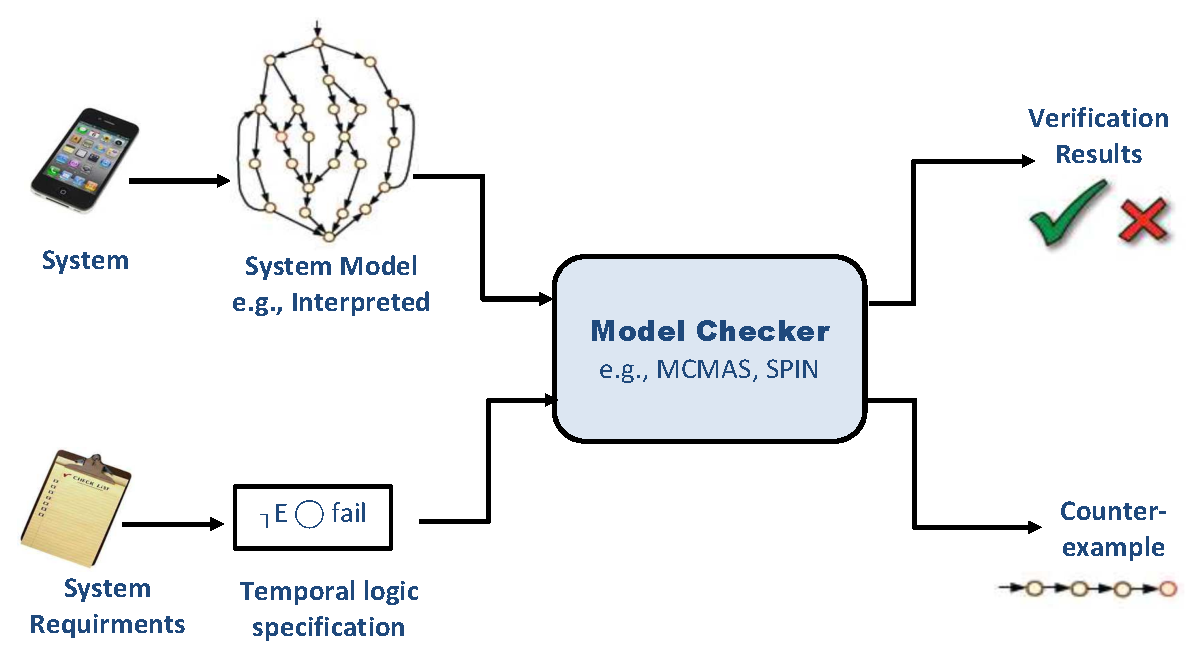
\includegraphics[width=12cm, height=7cm]{chap2/img/modelchecking1.eps}
                \end{center}
                \caption{Qualitative model checking overview}
                \label{fig:model-checking-cha2}
                \end{figure}

\subsection{Probabilistic Model Checking} \label{sec:pro-Model-Checking-cha2}

In addition to qualitative model checking, quantitative (or probabilistic) model checking techniques based on probabilistic model checkers have recently gained popularity \cite{Baier2008}. Probabilistic model checking is an automatic formal verification technique for the analysis of systems exhibiting stochastic behavior \cite{Hinton2006}. It offers the capability for interpreting the satisfiability of a given property in terms of quantitative results. In fact, the probabilistic model checking technique is similar to conventional model checking as discussed earlier. The major difference is that a probabilistic model contains additional information on the likelihood of transitions between states, or to be more specific, it can model probabilistic behavior. An overview of the probabilistic model checking procedure is given in Figure \ref{fig:prob-model-checking-cha2}. It shows that a probabilistic model checker takes as input a property and a model and delivers the result ``Yes'' or ``No'', or some probability.


\begin{figure}[t]
                \begin{center}
                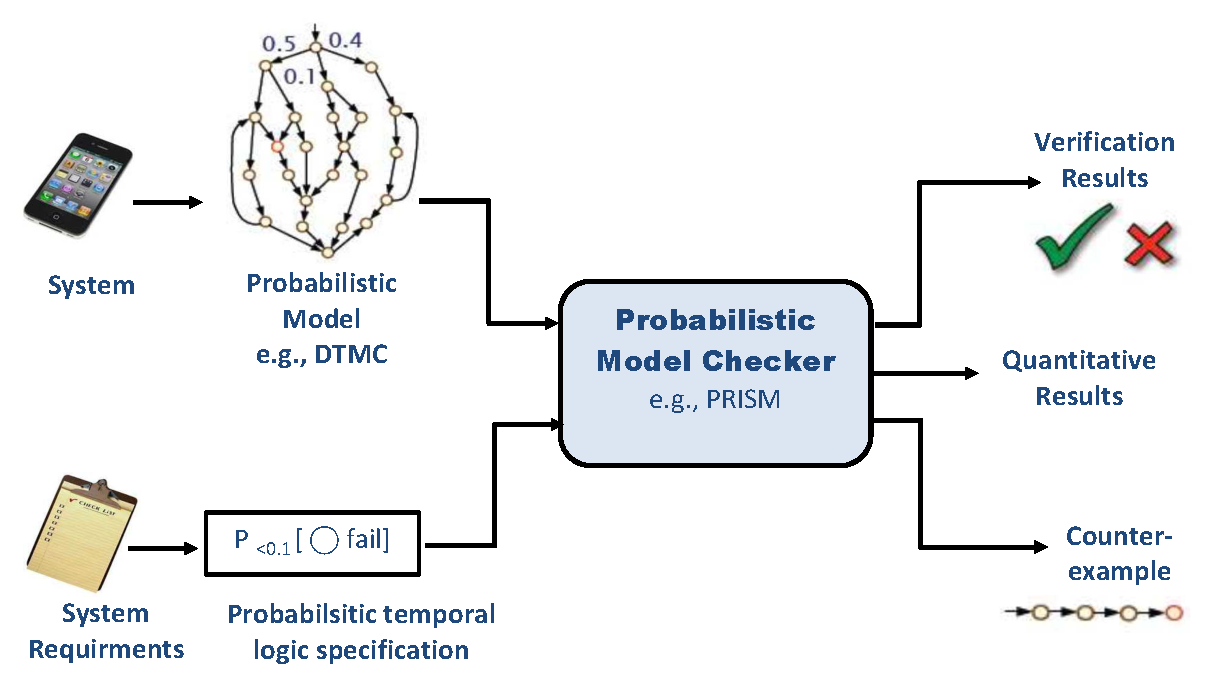
\includegraphics[width=12cm, height=7cm]{chap2/img/modelchecking2.eps}
                \end{center}
                \caption{Probabilistic model checking overview}
                \label{fig:prob-model-checking-cha2}
                \end{figure}


\subsection{Model Checking Tools}
There have been various model checking tools (also known as Model Checkers) in the literature. In this section, we review some of the most widely used model checkers.
\begin{itemize}

\item \textbf{MCMAS}\\
    MCMAS (Model Checker for Multi-Agent Systems) \cite{Lomuscio2006} is an OBDD-based symbolic model checker developed for the purpose of verifying epistemic properties of multi-agent systems. It supports branching-time temporal logic CTL. It also supports interpreted systems as an underling formalism for modeling target systems. The dedicated programming language used for describing a MAS in MCMAS is called ISPL (Interpreted Systems Programming Language). MCMAS was originally designed to handle the logic of knowledge CTLK and the branching-time temporal logic CTL. Recently, it has been extended by implementing some new algorithms that allow it to accept commitment formulae and hence to verify social commitments. The new extended version is called MCMASC (MCMAS for commitments). \cite{El-Menshawy2012}.


\item \textbf{NuSMV}\\
    NuSMV \cite{Cimatti2002}, an extension version of SMV \cite{McMillan1992}, is a well-known and widely trusted model checker. It is written in ANSI C language. As an input language, NuSMV accepts files written in SMV language. While the SMV tool was originally developed to implement the OBDD-based symbolic model checking for CTL, NuSMV implements also bounded model checking techniques for LTL -- in addition to the symbolic model checking techniques for CTL. This feature distinguishes it the most from SMV. Nevertheless, both SMV and NuSMV allow for a compact description of systems under consideration using modules, which may be composed to describe the evolution of states.



\item \textbf{SPIN}\\
    The SPIN \cite{Holzmann1997} model checker is one of the most used tools for tracing software defects in concurrent system designs. It was introduced in the 1980s at Bell Labs. Later, it has been made available to the public. The original version of SPIN has been continually under development and improvement. SPIN's programming language is called PROMELA. \cite{Holzmann2003} details the theoretical foundations of SPIN and presents the user manual. The main characteristics of SPIN are:

    $\diamond$ It is designed for the temporal logic LTL.\\
    $\diamond$ It is an automata-based model checker.\\
    $\diamond$ It implements various optimization strategies, including on-the-fly model checking and partial order reduction.

\item \textbf{PRISM} \\
    PRISM \cite{Kwiatkowska2002} stands for Probabilistic Symbolic Model Checker. It is the leading tool in the area of probabilistic model checking. The tool is widely used for checking probabilistic specifications over probabilistic models. The specifications can be expressed either in PCTL or in Continuous Stochastic Logic (CSL) \cite{Baier2008,Forejt2011}. Systems models can be described using the PRISM language as Discrete-Time Markov Chains (DTMCs), Continuous-Time Markov Chains (CTMCs), or Markov Decision Processes (MDPs). PRISM has been successfully used to analyse systems with a wide range of application domains, including communication and multimedia protocols, randomised distributed algorithms, security protocols, and many others.
    PRISM is the most appropriate tool for our work thanks to its capability of verifying probabilistic properties, and accepting formulae written in PCTL. Using PRISM, it is possible to either determine if a probability satisfies a given bound or obtain the actual value.

\item \textbf{MCK} \\
    MCK (stands for Model Checking Knowledge) is a model checker for the logic of knowledge, developed at the School of Computer Science and Engineering at the University of New South Wales \cite{Gammie2004}. It is implemented using OBDD-based symbolic algorithms. In the epistemic dimension, agents may use their observations in a variety of ways to determine what they know: observation alone, observation and clock, and perfect recall of all observations. The former way (observation alone) is to evaluate an agent's knowledge based merely on its current observation. The second way (observation and clock) is to compute an agent's knowledge based both on its current observation and the current clock value. The latter way (perfect recall of all observations) is to compute an agent's knowledge based on the complete record of all its observations.

    In the temporal dimension, specification formulae may use either linear time temporal logic (LTL), or the branching-time logic (CTL).
    Recently, MCK was extended by Huang et al. \cite{Huang2011} to permit the verification of knowledge in the presence of probabilistic behavior.





\end{itemize}

\section{Summary}\label{sec:summary-chap2}
In this chapter, we introduced the background and concepts needed for the rest of my thesis. As social commitments are the main focus of this research, it is important, again, to emphasis that the notion of ``social commitments'' we consider in this thesis is the communicative social commitments that are public and observable. In the next chapter, we propose a new probabilistic approach for handling social commitments in the presence of uncertainty.
